% !TEX TS-program = pdflatex
% !TEX encoding = UTF-8 Unicode

% This is a simple template for a LaTeX document using the "article" class.
% See "book", "report", "letter" for other types of document.

\documentclass[11pt,titlepage]{article} % use larger type; default would be 10pt

\usepackage[utf8]{inputenc} % set input encoding (not needed with XeLaTeX)

%%% Examples of Article customizations
% These packages are optional, depending whether you want the features they provide.
% See the LaTeX Companion or other references for full information.

%%% PAGE DIMENSIONS
\usepackage{geometry} % to change the page dimensions
\geometry{a4paper} % or letterpaper (US) or a5paper or....
% \geometry{margin=2in} % for example, change the margins to 2 inches all round
% \geometry{landscape} % set up the page for landscape
%   read geometry.pdf for detailed page layout information

\usepackage{graphicx} % support the \includegraphics command and options
\usepackage{titlepic}

% \usepackage[parfill]{parskip} % Activate to begin paragraphs with an empty line rather than an indent

%%% PACKAGES
\usepackage{booktabs} % for much better looking tables
\usepackage{array} % for better arrays (eg matrices) in maths
\usepackage{paralist} % very flexible & customisable lists (eg. enumerate/itemize, etc.)
\usepackage{verbatim} % adds environment for commenting out blocks of text & for better verbatim
\usepackage{subfig} % make it possible to include more than one captioned figure/table in a single float
% These packages are all incorporated in the memoir class to one degree or another...

%%% HEADERS & FOOTERS
\usepackage{fancyhdr} % This should be set AFTER setting up the page geometry
\pagestyle{fancy} % options: empty , plain , fancy
\renewcommand{\headrulewidth}{0pt} % customise the layout...
\lhead{}\chead{}\rhead{}
\lfoot{}\cfoot{\thepage}\rfoot{}

%%% SECTION TITLE APPEARANCE
\usepackage{sectsty}
\allsectionsfont{\sffamily\mdseries\upshape} % (See the fntguide.pdf for font help)
% (This matches ConTeXt defaults)

%%% ToC (table of contents) APPEARANCE
\usepackage[nottoc,notlof,notlot]{tocbibind} % Put the bibliography in the ToC
\usepackage[titles,subfigure]{tocloft} % Alter the style of the Table of Contents
\renewcommand{\cftsecfont}{\rmfamily\mdseries\upshape}
\renewcommand{\cftsecpagefont}{\rmfamily\mdseries\upshape} % No bold!

\newenvironment{changemargin}[3]{%
\begin{list}{}{%
\setlength{\topsep}{0pt}%
\setlength{\headsep}{#3}%
\setlength{\leftmargin}{#1}%
\setlength{\rightmargin}{#2}%
\setlength{\listparindent}{\parindent}%
\setlength{\itemindent}{\parindent}%
\setlength{\parsep}{\parskip}%
}%
\item[]}{\end{list}}

%Table Formatting
\usepackage{tabularx,hhline}
\usepackage{pbox}
\usepackage{booktabs}
\usepackage{makecell}
\usepackage{float}

%%% END Article customizations

%%% The "real" document content comes below...

\titlepic{\includegraphics[scale=0.60]{polimi_logo.jpg}}
\title{\textbf{I}ntegration \textbf{T}est \textbf{P}lan \textbf{D}ocument \\ \vspace{1cm} \large{Version 1.0}}
\author{Giorgio Pea(Mat. 853872), Andrea Sessa(Mat. 850082)}
\date{21/1/2016}

\begin{document}

\maketitle

\newpage

\tableofcontents

\newpage

\section{Introduction}

\subsection{Revision History}
	\begin{table}[h]
	  \centering
	  \begin{tabular}{lll}
	  \textbf{Date} & \textbf{Description} & \textbf{Authors} \\
	    21/01/2016 & Delivers of version 1.0 & Pea, Sessa
	  \end{tabular}
	\end{table}

\subsection{Purpose}
  The purpose of the integration test plan is to describe the necessary tests to verify that all the components(see \textbf{DD}, reference section)
  of MyTaxiServive are properly assembled.
  Integration testing ensures that the unit-tested components interact correctly. \newline
  
\subsection{Scope}
    The aim of this project is to develop MyTaxiService, a web/mobile application that
    makes easier and quicker taking taxies within the city’s borders. Thanks to MyTaxiService,
    anyone can request or book a taxi and get realtime information about how long
    it will take to be picked up or about the taxi’s current position and identification code.
    In addition to that, MyTaxiService provides an efficient way to allocate taxies by dividing
    the city in zones and using a queue based allocation system, in order to reduce the
    average waiting time and city’s traffic.\newline

\subsection{Terms Definition}
  \subsubsection{Glossary}
    \begin{itemize}
      \item \textbf{Mtaxi:} A taxi that joined MyTaxiService
      \item \textbf{User:} Refers to either a logged registered user or a generic user(see RASD)
      \item \textbf{MyTaxiService(B):} see RASD
      \item \textbf{Administrator:} see RASD
      \item \textbf{Mtaxi bad beahvior}: see RASD
    \end{itemize}
   
  \subsubsection{Acronyms}
    \begin{itemize}
      \item \textbf{DD:} Design Document
      \item \textbf{MVC:} Model View Controller
      \item \textbf{FIFO:} First In First Out
      \item \textbf{API:} Application Programming Interface
      \item \textbf{GUI:} Graphic User Interface
      \item \textbf{GPS:} Global Positioning System
      \item \textbf{CM:} Communication Manager
      \item \textbf{DB:} DataBase
     \end{itemize}

\subsection{Reference Documents}
  \begin{itemize}
   \item \textbf{[RASD]} Requirements and analisys specification document(RASD)
   \item \textbf{[DD]} Design Document(DD)
   \item \textbf{[A1]} Project's assignement number 1
   \item \textbf{[A2]} Project's assignement number 2
  \end{itemize}

\newpage

\section{Integration Strategy}

\subsection{Overview}
  In the first part of this section the components to be tested are mentioned,
  moreover the testing strategy is chosen and the integration testing order defined.\newline
  A more detailed specification for each test case is given in the third chapter.

\subsection{Entry Criteria}
  The main entry conditions for this phase is that each of the system components low level functions
  has been previously subjected to a unit test process. 

\subsection{Elements to be integrated}
  For a detailed description of each components function and interaction refer to the \textbf{DD} \newline
  Three main subsystem can be individuated in the general architecture of MyTaxiService:
  \begin{enumerate}
    \item \textbf{Client Side Components}
	  \begin{itemize}
	    \item MyTaxiServiceAppUser GUI
	    \item MyTaxiServiceMYT GUI
	    \item MyTaxiServiceWebUser GUI
	    \item MyTaxiServiceWebAdmin GUI
	    
	    \item MyTaxiServiceAppUser Communication Manager
	    \item MyTaxiServiceMYT Communication Manager
	    \item MyTaxiServiceWebUser Communication Manager
	    \item MyTaxiServiceWebAdmin Communication Manager
	  \end{itemize}
    
    \item \textbf{Server Side Components}
	  \begin{itemize}
	    \item Dispatcher
	    \item Request Manager
	    \item External Services Manager
	    \item Location Manager
	    \item Queue Manager
	    \item Request Receiver
	  \end{itemize}
    \item \textbf{Model Side Components}
	  \begin{itemize}
	   \item Data Manager
	  \end{itemize}

  \end{enumerate}


\subsection{Integration Testing Strategy}
  The strategy chosen for the integration of the components of the application is a grouped Bottom-Up integration: 
  for each subsystem S of MyTaxiService, its components are orchestrated together following a bottom-up approach, 
  when this procedure is finished a general integration of the subsystems of the application with each other is performed.\newline
  This integration testing strategy has been selected because it mimics very well the structure and the modularity of the software system.
  The bottom-up approach consists in integrating first those components that are at the low level of the component's dependency tree
  (see DD's component diagram).
  
\subsection{Sequence of Component/Function Integration} 
  In this section we included the integration sequence for the software components.\newline
  The arrows used in the following diagrams reflects the bottom-up integration sequence; in case the arrows does not fix a particular
  ordering in the integration of some components then the testing phase should give priority to the more critical or more complex component.
  
  \subsubsection{Software Integration Sequence}
    In the following diagram is represented the integration of the View subsystem\newline
    \begin{center}
      \includegraphics[scale=0.25]{Integration-1.png}
    \end{center}
    
\newpage

     \noindent In the following diagram is represented the integration of the Controller subsystem\newline
    \begin{center}
      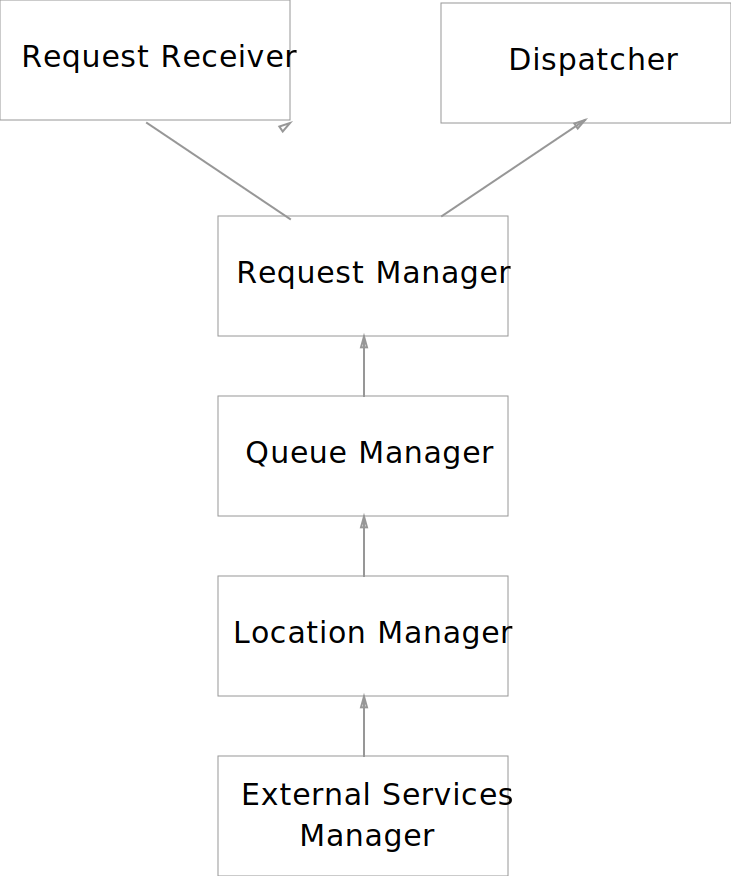
\includegraphics[scale=0.3]{Integration-2.png}
    \end{center}
  \subsubsection{Subsystem Integration Sequence}
    In the following diagram is rapresented the general integration sequence between the three subsystems.
    \begin{center}
      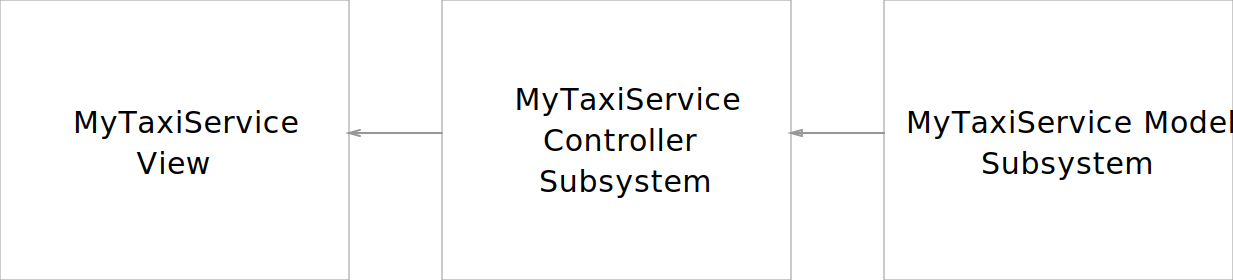
\includegraphics[scale=0.3]{Integration-3.png}
    \end{center}

\newpage
\section{Individual Step and Test Description}
  In this section is included the high level description for each step in the integration plan.
  Each test case correspond with one arrow in the previous diagram(see chapter 2)
  
  \subsection{Test Case I1}
  \begin{table}[ht!]
    \begin{tabular*}{16cm}{ll}
	\hline
	\textbf{Test Item(s)} & MyTaxiServiceApp CM $ \longrightarrow $ MyTaxiServiceApp GUI \\
	\hline
	\textbf{Input Specification} & Create the typical input for MyTaxiServiceApp CM\\
	\hline
	\textbf{Output Specification} & Check if the correct method are called in MyTaxiServiceApp GUI\\
	\hline
	\textbf{Environmental Needs} & N/A\\
	\hline
	\textbf{Purpose} & Verifies if MyTaxiServiceApp CM can handle user inputs \\
	\hline
    \end{tabular*}
  \end{table}
  
  \subsection{Test Case I2}
  \begin{table}[ht!]
    \begin{tabular*}{16cm}{ll}
	\hline
	\textbf{Test Item(s)} & MyTaxiServiceWeb CM $ \longrightarrow $ MyTaxiServiceWeb User GUI \\
	\hline
	\textbf{Input Specification} & Create the typical input for MyTaxiServiceWeb CM\\
	\hline
	\textbf{Output Specification} & \pbox{20cm}{Check if the correct method are called \\ in MyTaxiServiceWeb User GUI} \\
	\hline
	\textbf{Environmental Needs} & N/A\\
	\hline
	\textbf{Purpose} & \pbox{20cm}{Verifies if MyTaxiServiceWeb CM can handle user inputs \\ coming from the Web site} \\
	\hline
    \end{tabular*}
  \end{table}
  
  \subsection{Test Case I3}
  \begin{table}[ht!]
    \begin{tabular*}{16cm}{ll}
	\hline
	\textbf{Test Item(s)} & MYT CM $ \longrightarrow $ MYT GUI \\
	\hline
	\textbf{Input Specification} & Create the typical input for MYT CM\\
	\hline
	\textbf{Output Specification} & Check if the correct method are called in MYT GUI\\
	\hline
	\textbf{Environmental Needs} & N/A\\
	\hline 
	\textbf{Purpose} & \pbox{20cm}{Verifies if MYT CM can handle user inputs coming \\ from a taxi driver} \\
	\hline
    \end{tabular*}
  \end{table}
  
  \subsection{Test Case I4}
  \begin{table}[H]
    \begin{tabular*}{16cm}{ll}
	\hline
	\textbf{Test Item(s)} & MyTaxiServiceWeb Admin CM $ \longrightarrow $ MyTaxiServiceWeb Admin GUI \\
	\hline
	\textbf{Input Specification} & Create the typical input for MyTaxiServiceWeb Admin CM\\
	\hline
	\textbf{Output Specification} & \pbox{20cm}{Check if the correct method are called \\ in MyTaxiServiceWeb Admin GUI} \\
	\hline
	\textbf{Environmental Needs} & N/A\\
	\hline
	\textbf{Purpose} & \pbox{20cm}{Verifies if MyTaxiServiceWeb Admin CM can handle user inputs \\ coming from the admin interface} \\
	\hline
    \end{tabular*}
  \end{table}
  
  \subsection{Test Case I5}
  \begin{table}[ht!]
    \begin{tabular*}{16cm}{ll}
	\hline
	\textbf{Test Item(s)} & External Services Manager  $ \longrightarrow $ Location Manager \\
	\hline
	\textbf{Input Specification} & Create the typical input for External Services Manger\\
	\hline
	\textbf{Output Specification} & Check if the correct method are called into Location Manager\\
	\hline
	\textbf{Environmental Needs} & N/A\\
	\hline
	\textbf{Purpose} & \pbox{20cm}{Verifies can correctly provide location data to \\ the Location Manager} \\
	\hline
    \end{tabular*}
  \end{table}
  
  \subsection{Test Case I6}
  \begin{table}[ht!]
    \begin{tabular*}{16cm}{ll}
	\hline
	\textbf{Test Item(s)} & Location Manager $ \longrightarrow $ Queue Manager \\
	\hline
	\textbf{Input Specification} & Create the typical input for Location Manager\\
	\hline
	\textbf{Output Specification} & \pbox{20cm}{Check if Queue Manger driver receives the correct data \\ according to the input} \\
	\hline
	\textbf{Environmental Needs} & I5 succeeded \\
	\hline
	\textbf{Purpose} & \pbox{20cm}{Verifies if Location Manager produces and formats the location \\ data needed for the Queue Manager} \\
	\hline
    \end{tabular*}
  \end{table}
  
  \subsection{Test Case I7}
  \begin{table}[ht!]
    \begin{tabular*}{16cm}{ll}
	\hline
	\textbf{Test Item(s)} & Location Manager $ \longrightarrow $ Request Manager \\
	\hline
	\textbf{Input Specification} & Create the typical input for Location Manager \\
	\hline
	\textbf{Output Specification} & \pbox{20cm}{Check if Queue Manger driver receives the correct data \\ according to the input} \\
	\hline
	\textbf{Environmental Needs} & I5 succeeded \\
	\hline
	\textbf{Purpose} & \pbox{20cm}{Verifies if Location Manager produces and formats the location \\ data needed for the Request Manager} \\
	\hline
    \end{tabular*}
  \end{table}
  
  \subsection{Test Case I8}
  \begin{table}[ht!]
    \begin{tabular*}{16cm}{ll}
	\hline
	\textbf{Test Item(s)} & Queue Manager $ \longrightarrow $ Request Receiver \\
	\hline
	\textbf{Input Specification} & Create the typical input for Queue Manager \\
	\hline
	\textbf{Output Specification} & \pbox{20cm}{Check if Request Receiver driver receives the correct data \\ according to the input} \\
	\hline
	\textbf{Environmental Needs} & I6 and I7 succeeded\\
	\hline
	\textbf{Purpose} & \pbox{20cm}{Verifies if Queue Manager produces and formats the data needed \\ to manage a request} \\
	\hline
    \end{tabular*}
  \end{table}
  
  \subsection{Test Case I9}
  \begin{table}[H]
    \begin{tabular*}{16cm}{ll}
	\hline
	\textbf{Test Item(s)} & Request Manager $ \longrightarrow $ Dispatcher \\
	\hline
	\textbf{Input Specification} & Create the typical input for Queue Manager \\
	\hline
	\textbf{Output Specification} & Check if correct methods are called in Dispatcher \\
	\hline
	\textbf{Environmental Needs} & I6 and I7 succeeded\\
	\hline
	\textbf{Purpose} & \pbox{20cm}{Verifies if Request Manager produces the correct answers \\ according to the type of action requested} \\
	\hline
    \end{tabular*}
  \end{table}
  
  \subsection{Test Case I10}
  \begin{table}[ht!]
    \begin{tabular*}{16cm}{ll}
	\hline
	\textbf{Test Item(s)} & Data Manager $ \longrightarrow $ MyTaxiService Controller Subsystem \\
	\hline
	\textbf{Input Specification} & \pbox{20cm}{Create the typical memory situation in the DB \\ and create the typical input for MyTaxiService Controller Subsystem} \\
	\hline
	\textbf{Output Specification} & \pbox{20cm}{Check if correct methods are called in Data Manager \\ and the correct data are retrieved} \\
	\hline
	\textbf{Environmental Needs} & All the previous test phase has succeeded\\
	\hline
	\textbf{Purpose} & \pbox{20cm}{Verifies if the Controller Subsystem can \\ retrieve data from the DB system and if the Data Manager \\ can correctly handle data request coming from the Controller} \\
	\hline
    \end{tabular*}
  \end{table}
  
  \subsection{Test Case I11}
  \begin{table}[ht!]
    \begin{tabular*}{16cm}{ll}
	\hline
	\textbf{Test Item(s)} & MyTaxiService Controller Subsystem $ \longrightarrow $ MyTaxiService View Subsystem \\
	\hline
	\textbf{Input Specification} & Create the typical for MyTaxiService Controller \\
	\hline
	\textbf{Output Specification} & Check if correct data are retrieved by MyTaxiService View Subsystem \\
	\hline
	\textbf{Environmental Needs} & All the previous test phase has succeeded\\
	\hline
	\textbf{Purpose} & \pbox{20cm}{Verifies if the View Subsystem can correctly \\ interact with the Controller subsystem} \\
	\hline
    \end{tabular*}
  \end{table}

\newpage

\section{Tools and Test Equipment Required}
  In this section is included a set of suggestion about possible testing tools than could be used to perform the integration 
  testing describe above.\newline
  The selection of the tools depends on the selection of the programming language made by the developer.\newline
  If the chosen programming language is Java EE:
  \begin{enumerate}
   \item To perform the integration testing between the components the Java EE Arquillian Framework can be used;
	 it provides an environment in which the components under testing are inserted and tested. The specific 
	 test protocols will be specified and written in further documents.
   \item Manual testing could also be needed to simulate the input of the user in order to generate typical
	 input data used to integrate the various components.
  \end{enumerate}

\section{Program Stub and Test Data Required}
  In this section are included any specification of particular input data or component's stub/driver needed to 
  perform the integration steps describe in the previous section.\newline
  
  \noindent In order to perform the test case \textbf{I10} some anonymized user data should be inserted into the database system.\newline
  Appropriates drivers are needed to replace the two external systems: the GPS device and the Traffic Info Services
  These drivers should simulate external data needed to the External Services Manager to correctly perform the test case \textbf{I1} \newline
  In general more driver can be introduced: If the integration test phase is run in parallel with the developing phase then some components may no
  be already available for the integration test phase, such components will be replace with an appropriate driver.
  
  
\newpage
\section{Appendix}
  \subsection{Hours Of Work}
    \begin{itemize}
     \item Giorgio Pea: xxx hours
     \item Andrea Sessa: xxx hours
    \end{itemize}

  \subsection{Tools Used}
    \begin{itemize}
     \item  Atom/\LaTeX: to redact this document
    \end{itemize}
\end{document}
